\section{Performance Evaluation}
To evaluate the performance of \sink, we are concerned with (1) the overhead incurred by the semantic translation methods discussed in Section 4, (2) the message latency when crossing between different networks (e.g., the RTT of IP-to-NDN messages), and (3) the latency of messages traversing NDN bridges. Since directory updates happen infrequently and asynchronously, we did not measure the time to perform this task; we leave such evaluation to future work. To assess each of these measurements, we deployed a single bridge directory server that managed four (geographically) remote clients. Each of these hosts were running Ubuntu 12.10 and ran CCNx 0.81 and Python 3.1. All necessary cryptographic functions were implemented using Python standard libraries (i.e., the {\tt hmac} Python library). 

Measurements (1) and (2) were tested via scripts that issue a series of IP-to-NDN and NDN-to-IP requests and record the time to retrieve a response. More specifically, IP-to-NDN messages were generated and timed by a Python script using the {\tt httplib} library, and NDN-to-IP messages were generated and timed by a script that issues interests using the PyCCN library. The semantic overhead time was recorded by the gateway component itself (i.e., not by the test scripts). The resulting overhead of translating IP to NDN messages was determined to be approximately 0.00078s for interest names composed of one to five components. Similarly, the overhead of translating NDN to IP messages was slightly lower with an average time of 0.005s. Clearly, the overhead of both translations is negligible for sequential requests generated by a small number of clients\footnote{Due to a lack of resources, large-scale tests were not conducted to see how this overhead increased with request load.}. 

Since measurement (3) used the bridge component, we needed to test this using multiple machines. In this setup, two remote clients, $C_1$ and $C_2$, are connected to the central bridge directory and are used to issue and forward NDN interests. A script running on one client $C_1$ issued a series of NDN interests (via {\tt ccnpeek}) to be forwarded to the other client $C_2$ and satisfied by its set of connected NDN hosts, and the RTT to retrieve content for each invocation of {\tt ccnpeek} was recorded. This RTT includes the time to:
\begin{itemize} 
	\item Send the interest {\tt ccnx:/test/$r_i$} from the consumer script to the bridge on $C_1$ (where $r_i$ is the experiment iteration sequence number),
	\item Forward the interest from $C_1$ to $C_2$, 
	\item Re-issue the interest from $C_2$ to the producing application, 
	\item Retrieve the corresponding content from the producer at $C_2$,
	\item Sign and send the content from $C_2$ back to $C_1$, and
	\item Verify the content and send the result to the requesting consumer script.
\end{itemize}
The experimental setup and steps in this RTT calculation are shown in Figure \ref{fig:exp-bridge}.

\begin{figure}
\begin{center}
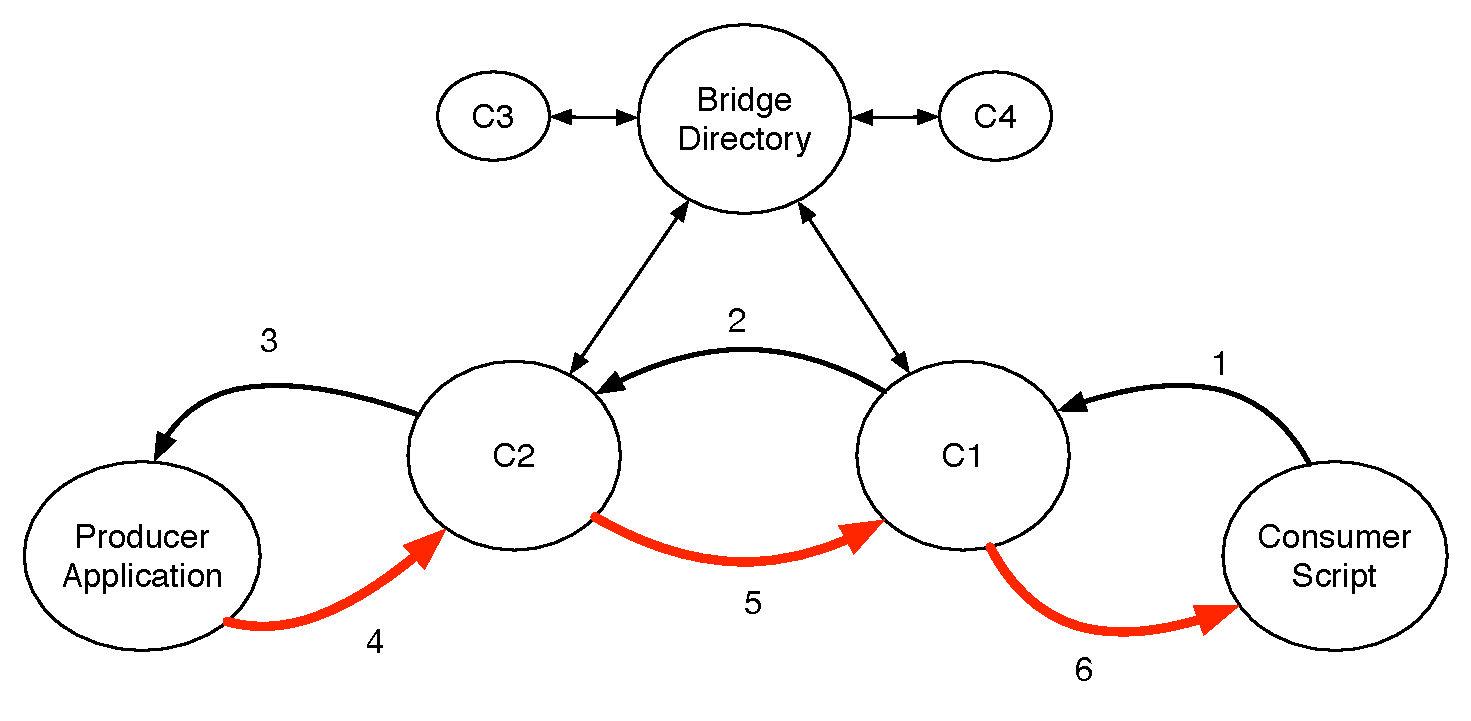
\includegraphics[scale=0.4]{./images/experiment.pdf}
\label{fig:exp-bridge}
\caption{Experimental setup for measuring the bridge component RTT.}
\end{center}
\end{figure}

The RTT results for measurements (2) and (3) when retrieving content of roughly 1MB and 10MB in size are shown in Figures \ref{fig:perf1} and \ref{fig:perf2}, respectively, and the RTT result for measurement (3) when retrieving content of 100MB is shown in Figure \ref{fig:perf3}, respectively. Our results indicate that IP-to-NDN and bridge message latencies were fairly consistent, whereas NDN-to-IP content retrieval incurred sporadic spikes in RTT. We attribute these anomalies to Python's thread synchronization primitives. We also note that the RTT times for the bridge are not worst-case in that they do include the preliminary TCP connection establishment and pair-wise key agreement overhead (using an appropriate Diffie Hellman group $\mathbb{Z}_p$, where $p$ is 1024 bits). Establishing the shared key takes approximately 0.186s\footnote{This average value was determined by timing the key establishment overhead for a small set of 10 experiments.} and the time to establish a TCP connection is negligible. It is also interesting to note the flucuations in the brige RTT time for large (100MB) content. This is due to the nature in which content was generated by the producing application. In particular, the producing application responds to all interests with \emph{random} bytes of data. In doing so, an arbitrary delay is also inserted so as to emulate real-world latency side-effects due to heavy loads, background application I/O, operating system context switches, etc. that could not be replicated in our small test environment. If this delay was removed, however, we would see much smoother RTT times for large pieces of content. 

\begin{figure}
\begin{center}
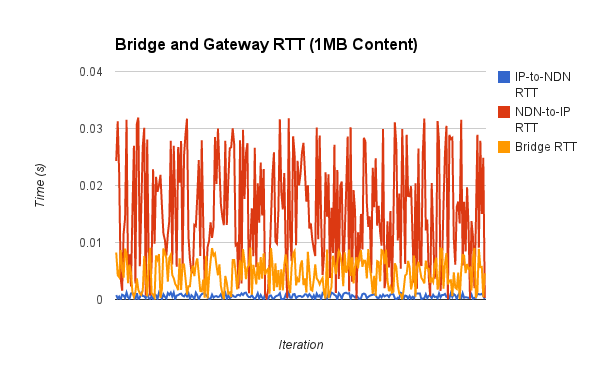
\includegraphics[scale=0.7]{./images/small.png}
\label{fig:perf1}
\caption{Average RTT times for IP-to-NDN, NDN-to-IP, and bridge messages when requesting content of approximately 1MB in size.}
\end{center}
\end{figure}

\begin{figure}
\begin{center}
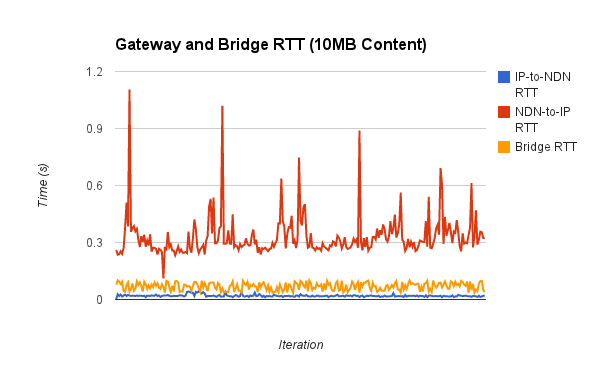
\includegraphics[scale=0.7]{./images/large.png}
\label{fig:perf2}
\caption{Average RTT times for IP-to-NDN, NDN-to-IP, and bridge messages when requesting content of 10MB in size.}
\end{center}
\end{figure}

\begin{figure}
\begin{center}
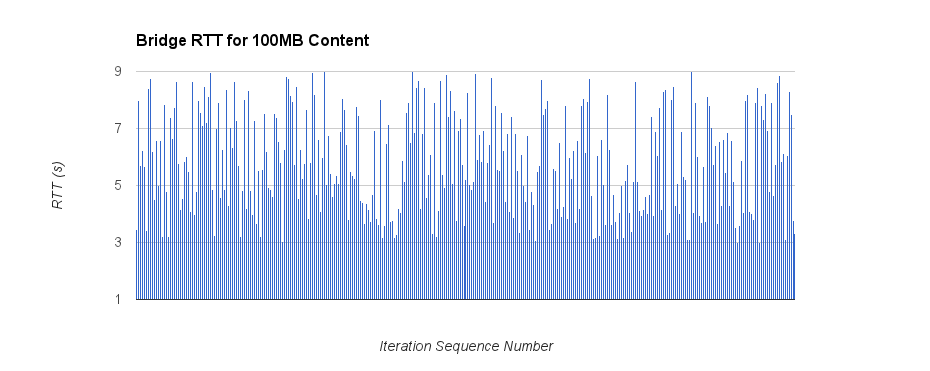
\includegraphics[scale=0.5]{./images/huge.png}
\label{fig:perf3}
\caption{Average RTT time for bridge messages when requesting content of 100MB in size.}
\end{center}
\end{figure}

% - test machine setup
% - experimental procedures and applications
% - link to source code
% - message translation overhead both ways
% - unidirectional and bidirectional RTT
% - bridge latency
% - say key generation and directory updates are asynchronous and one-time (don't happen a lot, so we didn't measure them)

